\documentclass[journal,12pt,twocolumn]{IEEEtran}
%

\usepackage{setspace}
\usepackage{gensymb}
\singlespacing

\usepackage{amsmath}
\usepackage{amsthm}
\usepackage{txfonts}
\usepackage{cite}
\usepackage{enumitem}
\usepackage{mathtools}
\usepackage{listings}
    \usepackage{color}                                            %%
    \usepackage{array}                                            %%
    \usepackage{longtable}                                        %%
    \usepackage{calc}                                             %%
    \usepackage{multirow}                                         %%
    \usepackage{hhline}                                           %%
    \usepackage{ifthen}                                           %%
  %optionally (for landscape tables embedded in another document): %%
    \usepackage{lscape}     
\usepackage{multicol}
\usepackage{chngcntr}
\renewcommand\thesection{\arabic{section}}
\renewcommand\thesubsection{\thesection.\arabic{subsection}}
\renewcommand\thesubsubsection{\thesubsection.\arabic{subsubsection}}

\renewcommand\thesectiondis{\arabic{section}}
\renewcommand\thesubsectiondis{\thesectiondis.\arabic{subsection}}
\renewcommand\thesubsubsectiondis{\thesubsectiondis.\arabic{subsubsection}}

% correct bad hyphenation here
\hyphenation{op-tical net-works semi-conduc-tor}
\def\inputGnumericTable{}                                 %%

\lstset{
%language=C,
frame=single, 
breaklines=true,
columns=fullflexible
}

\begin{document}
%


\newtheorem{theorem}{Theorem}[section]
\newtheorem{problem}{Problem}
\newtheorem{proposition}{Proposition}[section]
\newtheorem{lemma}{Lemma}[section]
\newtheorem{corollary}[theorem]{Corollary}
\newtheorem{example}{Example}[section]
\newtheorem{definition}[problem]{Definition}
\newcommand{\BEQA}{\begin{eqnarray}}
\newcommand{\EEQA}{\end{eqnarray}}
\newcommand{\define}{\stackrel{\triangle}{=}}

\bibliographystyle{IEEEtran}


\providecommand{\mbf}{\mathbf}
\providecommand{\pr}[1]{\ensuremath{\Pr\left(#1\right)}}
\providecommand{\qfunc}[1]{\ensuremath{Q\left(#1\right)}}
\providecommand{\sbrak}[1]{\ensuremath{{}\left[#1\right]}}
\providecommand{\lsbrak}[1]{\ensuremath{{}\left[#1\right.}}
\providecommand{\rsbrak}[1]{\ensuremath{{}\left.#1\right]}}
\providecommand{\brak}[1]{\ensuremath{\left(#1\right)}}
\providecommand{\lbrak}[1]{\ensuremath{\left(#1\right.}}
\providecommand{\rbrak}[1]{\ensuremath{\left.#1\right)}}
\providecommand{\cbrak}[1]{\ensuremath{\left\{#1\right\}}}
\providecommand{\lcbrak}[1]{\ensuremath{\left\{#1\right.}}
\providecommand{\rcbrak}[1]{\ensuremath{\left.#1\right\}}}
\theoremstyle{remark}
\newtheorem{rem}{Remark}
\newcommand{\sgn}{\mathop{\mathrm{sign}}}
\providecommand{\abs}[1]{\left\vert#1\right\vert}
\providecommand{\res}[1]{\Res\displaylimits_{#1}} 
\providecommand{\norm}[1]{\left\lVert#1\right\rVert}
\providecommand{\mtx}[1]{\mathbf{#1}}
\providecommand{\mean}[1]{E\left[ #1 \right]}
\providecommand{\fourier}{\overset{\mathcal{F}}{ \rightleftharpoons}}
\providecommand{\system}{\overset{\mathcal{H}}{ \longleftrightarrow}}
\newcommand{\solution}{\noindent \textbf{Solution: }}
\newcommand{\cosec}{\,\text{cosec}\,}
\providecommand{\dec}[2]{\ensuremath{\overset{#1}{\underset{#2}{\gtrless}}}}
\newcommand{\myvec}[1]{\ensuremath{\begin{pmatrix}#1\end{pmatrix}}}
\newcommand{\cmyvec}[1]{\ensuremath{\begin{pmatrix*}[c]#1\end{pmatrix*}}}
\newcommand{\mydet}[1]{\ensuremath{\begin{vmatrix}#1\end{vmatrix}}}
\newcommand{\proj}[2]{\textbf{proj}_{\vec{#1}}\vec{#2}}

\let\StandardTheFigure\thefigure
\let\vec\mathbf


\title{
Assignment - 1
}
\author{ Prakriti Sahu - SM21MTECH12009}
\maketitle
\newpage
\bigskip

\renewcommand{\thefigure}{\theenumi}
\renewcommand{\thetable}{\theenumi}

\section{Problem}
\renewcommand{\theequation}{\theenumi}
\begin{enumerate}[label=\thesection.\arabic*.,ref=\thesection.\theenumi]
\numberwithin{equation}{enumi}

\item Find the areas of the triangles formed by the triads of points (4,3), (1,-3), (-3,1), and (4,3), (-3,1), (1,-3) and explain the difference of signs in the two cases.

\solution
Let the points be-
\begin{align}
\vec{A} = \myvec{4\\3}, \vec{B} =\myvec{1\\-3}, \vec{C} =\myvec{-3\\1}
\end{align}
\begin{align}
\vec{P} =\myvec{4\\3}, \vec{Q} =\myvec{-3\\1}, \vec{R} =\myvec{1\\-3}   
\end{align}
We know area of a $\triangle$ with the vertices
$(x_{1},y_{1}),(x_{2},y_{2}),(x_{3},y_{3})$
can be given by:
\begin{align}
\label{eq:area_tri}
\mathbf{\Delta = \frac{1}{2}\begin{vmatrix}
x_{1} & y_{1} & 1\\ 
x_{2}& y_{2} & 1\\ 
x_{3} & y_{3} & 1
\end{vmatrix}}
\end{align}
$\therefore$ the area of $\Delta$ABC is
\\\\
$\Delta ABC=\frac{1}{2}\begin{vmatrix}
4 & 3 & 1\\ 
1 & -3 & 1\\ 
-3 &  1& 1
\end{vmatrix}$
\\\\\\
$\xrightarrow[]{R1\leftarrow R1+R2}\frac{1}{2}\begin{vmatrix}
5 & 0 & 2\\ 
1 & -3 & 1\\ 
-3 & 1 & 1
\end{vmatrix}$
\\\\\\
$\xrightarrow[]{R2\leftarrow R2-R3}\frac{1}{2}\begin{vmatrix}
5 & 0 & 2\\ 
4 & -4 & 0\\ 
-3 & 1 & 1
\end{vmatrix}$
\\\\\\
$\xrightarrow[]{C1\leftarrow C1+C2}\frac{1}{2}\begin{vmatrix}
5 & 0 & 2\\ 
0 & -4 & 0\\ 
-2 & 1 & 1
\end{vmatrix}$
\\\\\\
Expanding along the first row,
\\\\
$\Delta ABC=\frac{1}{2}\left [ 5((-4)1-0)-0+2(0-(-4)(-2)) \right ]$
\\
=$\frac{1}{2}\left [ 5(-4)+2(-8) \right ]$
\\$=\frac{1}{2}\left [ -20-16 \right ]$
\\
$=\frac{1}{2}\left ( -36 \right )$\\
\begin{align}
\label{eq:area_abc}
\therefore \Delta ABC=-18
\end{align}
\\
And, the area of $\Delta$PQR is
\\\\
$\Delta PQR=\frac{1}{2}\begin{vmatrix}
4 & 3 & 1\\ 
-3 & 1 & 1\\ 
1 & -3 & 1
\end{vmatrix}$
\\\\\\
$\xrightarrow[]{R2\leftrightarrow R3}\frac{-1}{2}\begin{vmatrix}
4 & 3 & 1\\ 
1 & -3 & 1\\ 
-3 & 1 & 1
\end{vmatrix}$\\\\\\
We notice that we get the exact same determinant as $\Delta ABC$, except for the difference in sign. $\therefore$ Substituting from \eqref{eq:area_abc}, we get
\begin{align}
\label{eq:area_pqr}
\Delta PQR=18    
\end{align}
\item Reason for difference in signs in the two cases:
\\\\
From \eqref{eq:area_abc} and \eqref{eq:area_pqr}, it is clear that the areas of both triangles have equal magnitude. The difference lies in the sign. This is because exchanging the $2^{nd}$ and $3^{rd}$ rows of determinant form of $\Delta ABC$ will get us the determinant form of $\Delta PQR$. And we know that exchanging two rows or columns of a determinant changes the sign.
\begin{figure}[!ht]
	\centering
	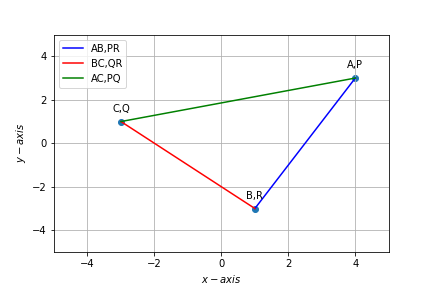
\includegraphics[width=\columnwidth]{triangle.png}
\end{figure}
\end{enumerate}
\end{document}









